\chapter{Estado del arte}
\label{ch:estado-arte}

\section{Inteligencia artificial}

El campo de la inteligencia artificial en la actualidad se encuentra en un estado de rápida evolución, con una infinidad de usos que se extiende por una gran variedad de sectores económicos y sociales. Su capacidad para analizar y procesar grandes cantidades de datos o para mejorar la eficiencia en distintas industrias han hecho que se trate de una tecnología en auge. El estudio de McKinsey \& Company (2022)~\cite{mckinsey2022ai} estima que el 50\% de las empresas ya usan IA en sus tareas diarias, donde destacan la optimización de servicios, la creación de productos y el análisis del servicio al cliente.

El informe AI Index Report 2024~\cite{AIIndex2024} muestra que la IA ya supera a las habilidades humanas en ciertas tareas, como en la clasificación de imágenes, con una precisión del 97\% respecto al 95\% de los humanos, o en juegos, como el ajedrez, donde supera consistentemente a los jugadores humanos.

Aunque sin duda, el mayor crecimiento en los dos últimos años corresponde a las herramientas relacionas con la \textit{Inteligencia Artificial Generativa (IAG)}. Esta rama se centra en crear modelos capaces de generar contenido, como conversaciones, imágenes, videos o música. Aprende de datos ya existentes y produce nuevos con características similares. En este ámbito destaca la empresa OpenAI, que cuenta con ChatGPT, capaz de generar texto lógico y actuar como chatbot, o con Dall-E, que puede generar imágenes en base a la descripción que se entregue. The state of AI in 2023: Generative AI's breakout year~\cite{mckinsey2023state} muestra que el 79\% de los encuestados dice haber tenido al menos alguna exposición a la IAG, lo que indica que es la herramienta de IA que más rápido está captando el interés del público general.

\begin{figure}[H]
    \centering
    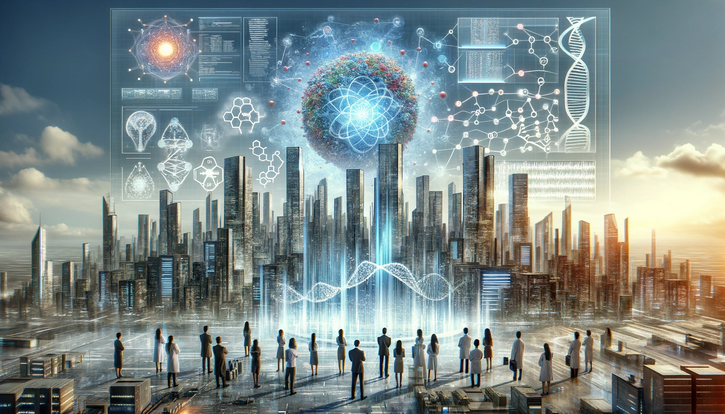
\includegraphics[width=0.5\textwidth]{figures/dall-e.png}
    \caption{Imagen generada con DALL-E 3.}
    \label{fig:dall-e}
\end{figure}

Existen numerosos proyectos pioneros actualmente en el campo de la IA. Entre los más destacados se encuentra AlphaFold de DeepMind, que utiliza IA para predecir las estructuras de proteínas, acelerando la investigación científica para la creación de nuevos medicamentos. Neuralink, por su parte, trabaja en un chip para comunicar directamente el cerebro humano con una computadora, mejorando los análisis neurológicos. En el ámbito de los vehículos autónomos, Waymo opera una flota de taxis sin conductor en Estados Unidos. Además, la medicina personalizada utiliza análisis de datos genéticos y médicos para diseñar tratamientos más efectivos para los pacientes.


\section{Algoritmos evolutivos}

Los algoritmos evolutivos han tenido varios proyectos que han marcado el desarrollo de esta tecnología. Los primeros acercamientos tuvieron lugar en las década de 1960 y 1970. Por un lado, Lawrence J. Fogel (1966)~\cite{fogel1966} comenzó a explorar la programación evolutiva, centrándose en la evolución de autómatas finitos. Uno de los primeros intentos de aplicar principios evolutivos a la informática. Por otro lado, Rechenberg (1973)~\cite{rechenberg1973} desarrolló estrategias de evolución para problemas de optimización técnica. Centradas en la selección y en la mutación, resultaron ser muy útiles para aplicarlas en la realidad.

Tras estos primeros pasos, John Holland fue fundamental para el desarrollo de los algoritmos genéticos. Su libro Adaptation in Natural and Artificial Systems del año 1975~\cite{holland1975} es básico para entender el funcionamiento de los mismos. Su trabajo se centró en la idea de que la evolución biológica podía ser simulada y utilizada para resolver problemas complejos en computación. Hacen uso de los operadores como la selección, el cruce o la mutación para evolucionar una población candidata de individuos hacia una mejor solución. Cada solución es evaluada según una función de fitness, que mide qué tan buena es la solución al problema en cuestión.

\begin{lstlisting}[caption=Algoritmo Genético]
INICIAR
    INICIALIZAR población
    EVALUAR fitness
    REPETIR HASTA CUMPLIR condición de parada:
        SELECCIONAR individuos
        CRUZAR padres
        MUTAR hijos
        EVALUAR individuos
        FORMAR nueva generación
    RETORNAR solución
FINALIZAR
\end{lstlisting}

Después de que Holland sentara las bases de los algoritmos genéticos, en los años siguientes fueron surgiendo estudios que hicieron evolucionar la rama. Varios de los más importantes fueron de John Koza~\cite{koza1992}~\cite{koza1994}, quien introdujo la programación genética, técnica usada para desarrollar automáticamente programas que realicen una tarea definida por el usuario. Se optimiza una población de individuos (programas) respecto a una función de aptitud. Koza probó su viabilidad para resolver problemas de robótica o de optimización.

Tras él han seguido surgiendo nuevas técnicas dentro de los algoritmos evolutivos. Entre ellas se puede destacar el desarrollo de los \textit{Algoritmos genéticos híbridos (AGH)}, que combinan los algoritmos genéticos con otras técnicas de optimización para mejorar las soluciones a los problemas complejos. Otro avance importante es el de la \textit{Programación genética cartesiana (CGP)}, que sustituye los árboles de busca usados en la programación genética tradicional por grafos dirigidos, lo que es muy útil, por ejemplo, en el diseño de circuitos electrónicos.

A lo largo de los años se han desarrollado distintos proyectos pioneros que han hecho uso de los algoritmos genéticos. Se puede destacar la misión de la NASA Space Technology 5 (ST5), donde ayudaron a la creación de una antena ultracompacta, con resultados extraordinarios. Además, también han sido empleados en áreas tan diversas como la economía o la bioingeniería, donde puede ayudar a tareas tan diversas como predecir movimientos del mercado o a modelar secuencias genéticas, respectivamente.


\section{Planificación nutricional mediante algoritmos evolutivos}

Los primeros acercamientos para intentar resolver problemas de optimización nutricional se dan en la década de 1940. George Stigler (1945)~\cite{stigler1945} planteó el problema de encontrar la dieta de menor coste que cumpliese con unos objetivos nutricionales. Al no poseer ordenadores, utilizó técnicas manuales.

El problema fue formalmente resuelto dos años después por Jack Laderman usando programación lineal. Fue capaz de calcular la combinación de alimentos que cumpliese con los requisitos económicos y nutricionales. Con esto se demostró la utilidad de técnicas computacionales en tareas de optimización.

Tras los estudios de Holland, en la década de los 70 y 80 empezaron a aparecer distintos trabajos que hacían uso de los algoritmos genéticos para resolver problemas de optimización. Si bien estos no estaban relacionados directamente con la planificación nutricional, sí que sentaron las bases para la resolución de este tipo de problemas. Se puede destacar los trabajos de Scott Kirkpatrick et al. (1983)~\cite{kirkpatrick1983} y de David E. Goldberg (1989)~\cite{goldberg1989}, donde hacen uso de estos algoritmos para optimizar problemas con múltiples restricciones.

Fue a partir de la década de los 2000 cuando aparecieron muchos de los trabajos y estudios relacionados con la planificación nutricional.

EL trabajo de Kahraman y Seven (2005)~\cite{kahraman2005} desarrolla un algoritmo genético bi-objetivo que propone comidas diarias saludables basados en parámetros especificados por el usuario a través de la interfaz gráfica, como la edad o el género. Optimiza la selección de platos para cumplir con restricciones nutricionales, minimizar costos y maximizar las preferencias del usuario.

Kaldirim y Köse (2006)~\cite{kaldirim2006} hacen una continuación de este trabajo. Hace uso del algoritmo multiobjetivo NSGA-II para gestionar de manera separada los objetivos de coste mínimo y máxima satisfacción, mejorando el manejo de restricciones nutricionales con la inclusión de límites. También presenta una mejora a la interfaz gráfica del anterior proyecto.

El estudio de Kashima et al. (2009)~\cite{kashima2009} presenta una interesante diferencia respecto a trabajos anteriores. Busca crear una aplicación web para ofrecer un servicio para compartir menús, creados para cada individuos haciendo uso de algoritmos genéticos, entre una comunidad de usuarios con el objetivo de fomentar los hábitos saludables.

Heinonen y Juuso (2016)~\cite{heinonen2016} presentan el uso que le dan a los algoritmos genéticos en su aplicación Nutri-Flow, un software que proporciona guías dietéticas personalizadas.

Ya en esta década han seguido surgiendo proyectos pioneros que hacen evolucionar la rama de los algoritmos genéticos.

En el trabajo realizado por Kilicarslan et al. (2021)~\cite{KILICARSLAN2021102231} se propone modelos híbridos que combinan algoritmos genéticos con aprendizaje profundo para la predicción y clasificación de anemias nutricionales. Optimiza los parámetros de los algoritmos de aprendizaje mediante computación evolutiva, lo que mejora la precisión de la planificación nutricional del paciente.

Joanne B. Cole y Rosita Gabbiannelli (2022)~\cite{cole2022} muestran cómo se puede integrar la IA con el análisis genético para la nutrición personalizada del paciente. Basándose en el perfil genético y otros datos biométricos, es posible, junto a los algoritmos evolutivos, generar planes de comida y predicciones sobre la salud del usuario.




